\documentclass[a4paper,12pt]{report}

% Packages
\usepackage{graphicx}
\usepackage{amsmath}
\usepackage{geometry}
\usepackage{fancyhdr}
\usepackage{setspace}
\usepackage{titlesec}  % For title formatting
\usepackage{hyperref}
\usepackage{xcolor}
\graphicspath{ {./images/} }

\usepackage[Lenny]{fncychap}
\ChNameUpperCase
\ChNumVar{\fontsize{40}{42}\usefont{OT1}{ptm}{m}{n}\selectfont}
\ChTitleVar{\Large\sc}

\geometry{margin=1in}
\setstretch{1.5}

\usepackage{listings}

\definecolor{codegreen}{rgb}{0,0.6,0}
\definecolor{codegray}{rgb}{0.5,0.5,0.5}
\definecolor{codepurple}{rgb}{0.58,0,0.82}
\definecolor{backcolour}{rgb}{0.95,0.95,0.92}

\lstdefinestyle{mystyle}{
    backgroundcolor=\color{backcolour},   
    commentstyle=\color{codegreen},
    keywordstyle=\color{magenta},
    numberstyle=\tiny\color{codegray},
    stringstyle=\color{codepurple},
    basicstyle=\ttfamily\footnotesize,
    breakatwhitespace=false,         
    breaklines=true,                 
    captionpos=b,                    
    keepspaces=true,                 
    numbers=left,                    
    numbersep=5pt,                  
    showspaces=false,                
    showstringspaces=false,
    showtabs=false,                  
    tabsize=2
}

\lstset{style=mystyle}



% Header and Footer
\pagestyle{fancy}
\fancyhf{}
\fancyhead[L]{OverseerAI}
\fancyhead[R]{\thepage}

% Title Formatting
\titleformat{\section}{\normalfont\Large\bfseries}{\thesection}{1em}{}


% Cover Page
\title{
    
\includegraphics[width=0.40\textwidth]{images/logo_overseerai.png}
    
    \textbf{\Huge OverseerAI} \\
    \vspace{1cm} % Adjust vertical space
    \large Laurea di Informatica L-31 all'Università di Salerno \\
    \large Corso di Fondamenti di Intelligenza Artificiale \\
    \vspace{0.5cm} % Adjust vertical space
    \small \textit{Gennaio 2025} \\
    \vspace{3cm}
    \textbf{Created by: }{\large Antonio Maiorano} \\
    \vspace{0.5cm}
    \textbf{Supervised by: }{\large Prof. Fabio Palomba}
}
\date{}

\tolerance=1
\emergencystretch=\maxdimen
\hyphenpenalty=10000
\hbadness=10000

\begin{document}

% Title Page
\maketitle
\thispagestyle{empty}
\newpage

% Table of Contents
\renewcommand*\contentsname{\hfill Indice \hfill}
% Start page numbering from the Table of Contents
\setcounter{page}{1}  % Start counting from 1
\tableofcontents
\newpage

\begingroup%
\makeatletter%
\let\clearpage\relax% Stop LaTeX from going to a new page; and
\vspace*{\fill}%
\vspace*{\dimexpr-50\p@-\baselineskip}% Remove the initial (default) 50pt gap (plus 1 line)
\chapter{Definizione del problema}
\vspace*{\fill}%
\endgroup
\newpage


\section{Introduzione}
YouTube è una delle piattaforme di condivisione video più utilizzate al mondo. Tuttavia, con l'aumento dei contenuti, sono cresciuti anche i tentativi di truffa, certe volte mascherati con il metodo "\textit{fare tanto, dando poco}".\\
Per semplicità di analisi, i contenuti "truffa" sono una generalizzazione di tutti quei contenuti che portano l'utente finale a consumare contenuti che sono descritti in modo fuorviante e/o sbagliato, si includono dunque i contenuti che reindirizzano ad altri contenuti esterni alla piattaforma per lo stesso obiettivo.\\
Queste problematiche sono ora piu' presenti che mai a causa della rapida crescita della presenza online dei contenuti AI-Made (le cosiddette "Money Farm") e pubblicità sponsorizzate da individui singoli con intenzioni a volte poco chiare, e poco legittime.

\section{Obiettivi}
L'obiettivo principale di questo progetto è quello di evitare il piu' possibile un contatto diretto con questi contenuti-truffa creando un modello di Machine Learning in grado di classificare i titoli dei video.

\section{Specifica P.E.A.S.}
\subsection{Performance}
La misura delle prestazioni del modello:
\begin{itemize}
    \item Correttezza di classificazione dei titoli.
\end{itemize}

\subsection{Environment}
Descrizione degli elementi che formano l'ambiente in cui il modello opererà:
\begin{itemize}
    \item Dataset sintetico di titoli creati con l'aiuto di Large Language Models, i cui elementi saranno descritti di seguito (applicati limiti derivanti dalla piattaforma stessa).
\end{itemize}

\subsection{Actuators}
Gli attuatori che prenderanno le decisioni nel modello:
\begin{itemize}
    \item Classificatore che determinerà l'appartenenza di un titolo ad una delle due categorie.
\end{itemize}

\subsection{Sensors}
I sensori attraverso cui il modello riceve le percezioni su cui opererà:
\begin{itemize}
    \item La finestra di input.
\end{itemize}

\section{Caratteristiche dell'Ambiente}
\begin{itemize}
    \item \textbf{Osservabilità:} Parzialmente osservabile.
    \begin{itemize}
        \item Il modello può osservare ed analizzare solo le caratteristiche del video e non il contenuto del video stesso.
    \end{itemize}
    \item \textbf{Determinismo:} Parzialmente stocastico.
    \begin{itemize}
        \item Presenza di ambiguità e rumore all'interno delle caratteristiche in analisi.
    \end{itemize}
    \item \textbf{Episodicità:} Episodico.
    \begin{itemize}
        \item Ogni titolo viene esaminato indipendentemente dagli altri
    \end{itemize}
    \item \textbf{Dinamismo:} Statico.
    \begin{itemize}
        \item I dati usati dal modello sono costanti, e non subiscono cambiamenti.
    \end{itemize}
    \item \textbf{Tipo di agente:} Singolo agente.
    \begin{itemize}
        \item Vi è un solo agente ad analizzare i titoli.
    \end{itemize}
\end{itemize}

\newpage

\section{Metodologia}
La valutazione della metodologia di approccio al problema in analisi è stata fatta tra i modelli di Ingegneria del Machine Learning \textbf{CRISP-DM} e \textbf{TDSP}, dove è stato scelto il primo, data la non necessità di suddivisioni e validazioni temporali del progetto presenti nel secondo.

\subsection{CRISP-DM}
Le fasi che verranno percorse sono:
\begin{enumerate}
    \item Business Understanding.
    \item Data Understanding.
    \item Data Preparation.
    \item Data Modeling.
    \item Evaluation.
\end{enumerate}

\newpage

\begingroup%
\makeatletter%
\let\clearpage\relax% Stop LaTeX from going to a new page; and
\vspace*{\fill}%
\vspace*{\dimexpr-50\p@-\baselineskip}% Remove the initial (default) 50pt gap (plus 1 line)
\chapter{Business Understanding}
\vspace*{\fill}%
\endgroup
\newpage

\section{Determinare gli Obiettivi di Business}
Il primo passo per la creazione di OverseerAI, è capire cosa esso deve essere, come deve esserlo e come esso deve arrivare ad essere cio' che è stato descritto di esso.\\
Partendo dalla radice: il problema in analisi è un problema di classificazione, come vedremo più avanti esso è nello specifico di \textbf{classificazione binaria}.
\subsection{Background}
Esistono molti sistemi di "Auto-Flagging", o di Moderazione automatica, YouTube stesso ne ha almeno uno!\\
...Il problema è che i contenuti moderati sono solo quelli degli utenti, ad esempio le pubblicità non sono moderate, per qualche ragione di Business di Google.\\
Un sistema esistente (e dignitosamente più funzionante dell'esempio appena esplicitato) da cui OverseerAI potrebbe prendere spunto:
\begin{itemize}
    \item \textbf{La moderazione automatica del social media TikTok} 
\end{itemize}
Il suddetto sistema funziona sulla base di un algoritmo (Closed-Source) che modera i contenuti in modo automatico basandosi su similarità con i contenuti di allenamento, che, nel caso di TikTok, possono essere Hashtags riconosciuti come pericolosi (la ricerca sulla piattaforma di tali Hashtags porta zero risultati), oppure delle parole presenti nella descrizione che sono anche essere già conosciute come pericolose.\\
Con grande probabilità esso utilizza anche un algoritmo per l'analisi dei contenuti.

\subsection{Obiettivi di Business}
Basandoci sulle informazioni raccolte, OverseerAI dovrà analizzare TUTTI i contenuti di YouTube, in particolare i loro titoli. Assieme ad essi si potrebbe analizzare la presenza di link all'interno della descrizione, che sono la maggior parte delle volte usati per truffare e rubare dati alle persone ignare.\\
Ovviamente quest'ultimo puo' facilmente essere un falso positivo, in quanto ci sono anche canali leciti che usano i link per aiutare le persone a connettere con loro attraverso altri social media.

\newpage
\section{Criteri di successo}
Gli obiettivi, non per ordine di importanza, di OverseerAI dunque sono:
\begin{itemize}
    \item \textbf{Un corretto riconoscimento dei contenuti intenzionati a truffare}
    \item \textbf{Un corretta classificazione dei contenuti normali come leciti}
    \item \textbf{Evitare di creare bias con chi ha link nei propri contenuti}
\end{itemize}
Ovviamente, assieme ad essi, c'è anche il criterio di aver sventato delle truffe!

\section{Limiti}
A causa di un recente cambiamento nella piattaforma di Youtube, vi è un limite alla consumazione di contenuti, soprattutto se l'utente non ha eseguito il Login.\\
Inoltre, anche lo scraping stesso del sito è stato limitato di molto (\href{https://web.archive.org/web/20240807161716/https://www.tomsguide.com/ai/nvidia-accused-of-scraping-80-years-worth-of-of-videos-daily-to-train-ai-models-what-you-need-to-know}{\color{blue}{causa}}).\\
Volendo evitare un aumento esponenziale della complessità del progetto, dovuto anche al dover ricercare manualmente le entries da aggiungere al dataset, e volendo rimanere in un'ottica più generale, l'intenzione iniziale di usare dati reali ottenuti dalla piattaforma stessa è stata accantonata,  ai dati creati sinteticamente tramite l'uso di LLMs e tramite l'utilizzo di scripts python di potenziamento.

\section{Tecnologie Usate}
Le principali tecnologie usate sono:
\begin{itemize}
    \item I \textbf{LLMs} come tool di supporto;
    \item \textbf{Python} come linguaggio di programmazione;
    \begin{itemize}
        \item Diverse librerie usate per le funzioni critiche, tra le quali \texttt{\color{red}{pandas}} per alcune funzioni base eseguite sul Dataset, \texttt{\color{red}{sklearn}} per le funzioni di Machine Learning, etc...
    \end{itemize}
\end{itemize}

\newpage

\begingroup%
\makeatletter%
\let\clearpage\relax% Stop LaTeX from going to a new page; and
\vspace*{\fill}%
\vspace*{\dimexpr-50\p@-\baselineskip}% Remove the initial (default) 50pt gap (plus 1 line)
\chapter{Data Understanding}
\vspace*{\fill}%
\endgroup
\newpage

\section{Ottenimento dei Dati}
Come descritto in precedenza, a causa di alcuni limiti non ci sarà possibile utilizzare dati reali.\\
Al loro posto, utilizzeremo dei dati creati sinteticamente tramite l'uso di LLMs.\\
Dopo l'istruzione, del suddetto, a riguardo del problema in esame, e del contesto ad esso relativo, non vi è granchè bisogno di fare Prompt Engineering: richiedendo semplicemente la generazione delle istanze, e per ogni iterazione essere sicuri di non averne di ripetute per evitare problemi, esso ne genererà continuamente.\\
Le istanze generate sono istanze di struttura CSV, dove vi sono solo due features:
\begin{itemize}
        \item Il \textbf{titolo}, \texttt{\color{red}{title}};
        \item Una \textbf{etichetta, Target Feature del dataset}, \texttt{\color{red}{label}}, che può essere "scam" o "legit", e determina se un video è truffaldino o meno;
        \item Una \textbf{descrizione}, \texttt{\color{red}{description}}, che contiene testo e può contenere link al suo interno.
\end{itemize}
Le istanze sono generate solo con queste tre features causa la tipologia delle features stesse: sono strettamente collegate e devono avere senso nel contesto dell'istanza, dunque non possono essere generate come le altre features, invece indipendenti tra loro.\\
Inoltre le istanze verranno generate in inglese per semplicità.

\section{Miglioramento del Dataset}
\subsection{Aggiunta di features}
I dati creati sinteticamente mancano di alcune features collegate ai contenuti.\\
Ovviamo a questo problema creando da zero dei dati realistici, con funzioni randomiche basate su osservazioni soggettive dei casi reali.\\
Le features riguardante i contenuti che verranno create sono:
\begin{itemize}
        \item I \textbf{mi piace} come \texttt{\color{red}{likes}};
        \item I \textbf{non mi piace} come \texttt{\color{red}{dislikes}};
        \item L' \textbf{ora di caricamento} come \texttt{\color{red}{upload\_hour}};
        \item I \textbf{commenti} come \texttt{\color{red}{comments}}.
\end{itemize}
Dopo aver creato le features nel dataset, procederemo ad assegnare ad ogni istanza dei valori ad essi riguardanti.\\

\begin{lstlisting}[language=Python]
import pandas as pd
import random
import numpy as np

def add_features(df):
    df['upload_hour'] = np.random.randint(0, 24, df.shape[0])
    df['likes'] = np.random.randint(0, 100001, df.shape[0])
    df['dislikes'] = np.random.randint(0, 10001, df.shape[0])
    df['comments'] = np.random.randint(0, 10001, df.shape[0])
\end{lstlisting}

\subsection{Aggiunta di rumore}
Il dataset risultante è vicino ad alla realtà, ma per renderlo ancor più realistico aggiungiamo del rumore nei dati, molto spesso presente in qualsiasi dataset.\\
Per il 3\% delle istanze del dataset, viene introdotto rumore per la feature "titolo", e la tipologia di rumore viene introdotto randomicamente nella scelta di uno dei seguenti:
\begin{itemize}
        \item Sostituzione di caratteri con caratteri casuali;
        \item Aggiunta di caratteri speciali;
        \item Mescolamento dei caratteri originali;
        \item Testo generico di errore.
\end{itemize}
Per il 5\% delle istanze del dataset, viene introdotto rumore per una delle features tra "upload\_hour", "likes", "dislikes" o "comments", immettendo valori vuoti "NaN".\\
Per il 5\% delle istanze del dataset, viene introdotto rumore per le features "likes" e "dislikes" immetendo valori anomali, in questo caso valori assurdi.
\\
\begin{lstlisting}[language=Python]
import pandas as pd
import random
import numpy as np
def add_noise(df):
    def corrupt_title(title):
        if pd.isnull(title):
            return title

        noise_methods = [
            lambda x: ''.join(random.choice(string.ascii_letters + string.digits + string.punctuation) for _ in range(len(x))),
            lambda x: x + ''.join(random.choices(string.punctuation, k=5)), 
            lambda x: ''.join(random.sample(x, len(x))),
            lambda x: '###ERROR###'
        ]

        return random.choice(noise_methods)(title)

    noise_indices = df.sample(frac=0.03).index
    df.loc[noise_indices, 'title'] = df.loc[noise_indices, 'title'].apply(corrupt_title)

    for col in ['upload_hour', 'likes', 'comments']:
        df.loc[df.sample(frac=0.05).index, col] = np.nan

    noise_indices = df.sample(frac=0.05).index
    (`len(noise_indices)`)
    df.loc[noise_indices, 'likes'] = np.random.randint(1000000, 10000000, len(noise_indices))
    df.loc[noise_indices, 'dislikes'] = np.random.randint(500000, 1000000, len(noise_indices))

    return df
\end{lstlisting}
\newpage

\begingroup%
\makeatletter%
\let\clearpage\relax% Stop LaTeX from going to a new page; and
\vspace*{\fill}%
\vspace*{\dimexpr-50\p@-\baselineskip}% Remove the initial (default) 50pt gap (plus 1 line)
\chapter{Data Preparation}
\vspace*{\fill}%
\endgroup
\newpage

\section{Preparazione del dataset}
Il dataset in uso presenta tipi diversi di rumore: su tutte le features, ci sono dei valori anomali che potrebbero creare problematiche anche rilevanti durante la creazione e l'utilizzo del modello.\\
Prima di passare dunque alla suddetta fase, il dataset deve essere pulito.\\
Inoltre, i valori numerici potrebbero essere problematici in fase di training, in quanto risulta avere valori senza un contesto: un esempio semplice può essere \texttt{\color{red}{upload\_hour}} che è un valore numerico con un contesto specifico, ovvero quello delle ore in una giornata, e non ha dunque senso unicamente come numero e fuori contesto.\\
Infine, i testi, nella forma attuale, devono essere normalizzati per avere una forma non ambigua e facilitare la fase di training.

\section{Data cleaning}
\subsection{Valori numerici}
Le prime features del processo di pulizia sono \texttt{\color{red}{upload\_hour}}, \texttt{\color{red}{likes}}, \texttt{\color{red}{dislikes}} e \texttt{\color{red}{comments}}.\\
In esse, abbiamo due problematiche principali:
\begin{itemize}
        \item La presenza di valori mancanti;
        \item La presenza di valori assurdi/anomali.
\end{itemize}
La prima problematica si risolve con una semplice \textbf{Imputazione statistica}, usando come funzione la Mediana.
\begin{lstlisting}[language=Python]
import pandas as pd
import re
# ...NLP libraries
def clean_dataset(df):
    def value_imputation(df, column):
        median_value = df[column].median()
        df[column].fillna(median_value, inplace=True)
        return df
    for col in ['upload_hour', 'likes', 'dislikes', 'comments']:
        df = value_imputation(df, col)
\end{lstlisting}
La seconda problematica si risolve utilizzando una funzione statistica di \textbf{Range Interquartile} (IQR), i valori in analisi che non rispettano il suddetto vengono rimpiazzati con il valore mediano della colonna in cui esso si trova.
\\
\[
\text{IQR} = Q_3 - Q_1
\]
\[
\textbf{dove}
\]
\[
Q_1 = \text{termine in posizione } \frac{n + 1}{4}
\]
\[
Q_3 = \text{termine in posizione } \frac{3(n + 1)}{4}
\]
\begin{figure}[h]
\centering
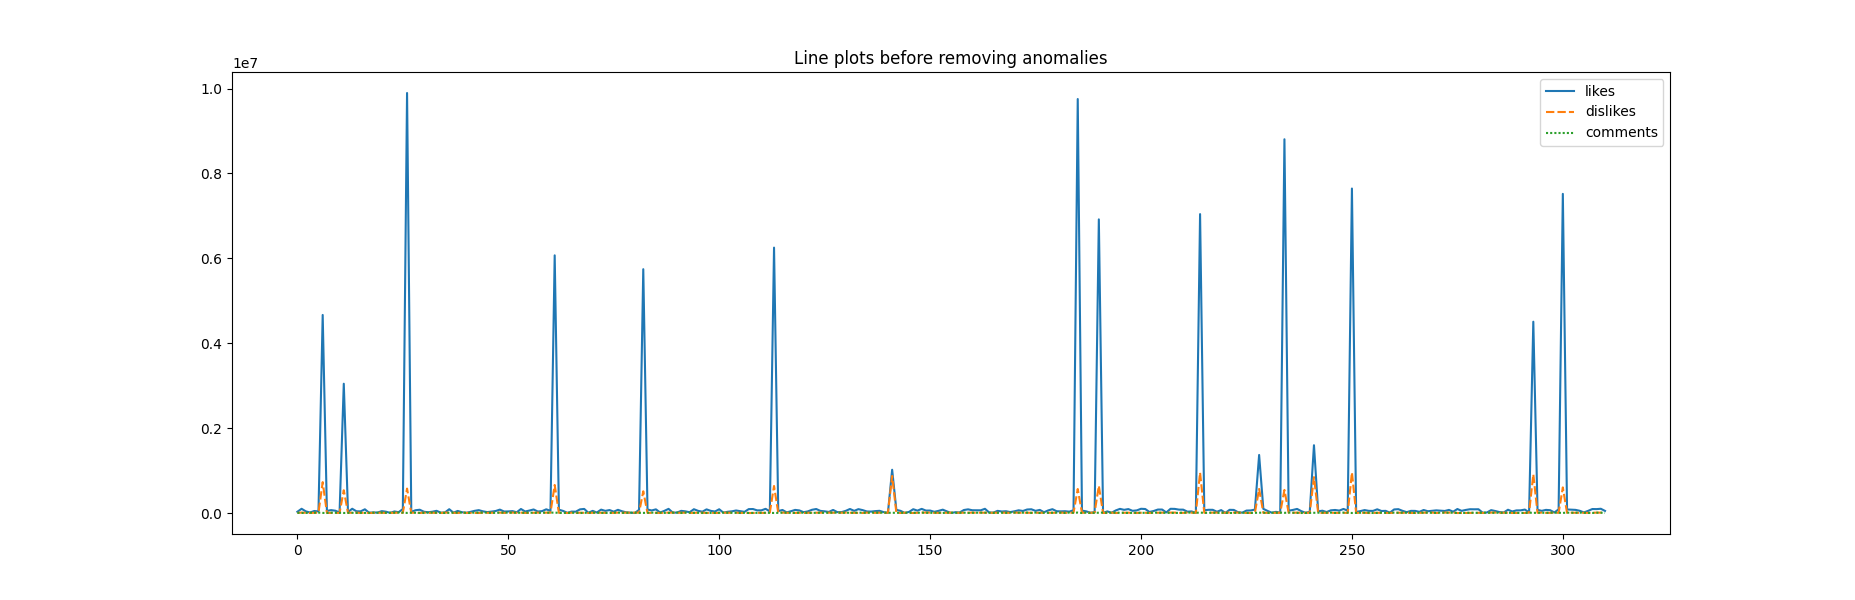
\includegraphics[width=\textwidth]{before_IQR.png}
\caption{Prima della rimozione degli Outliers (anomalie)}
\end{figure}
\begin{figure}[h]
\centering
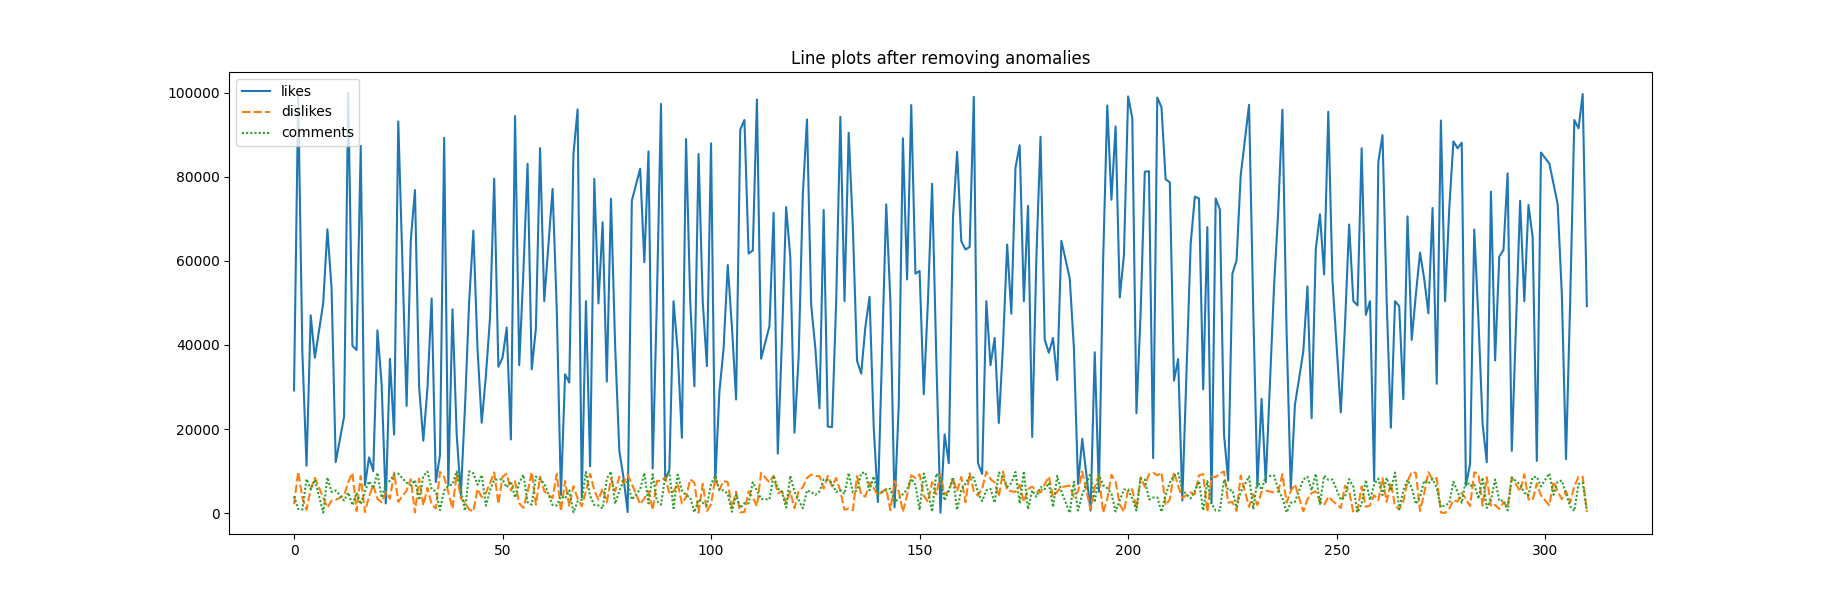
\includegraphics[width=\textwidth]{after_IQR.png}
\caption{Dopo la rimozione degli Outliers (anomalie)}
\end{figure}
\newpage
\begin{lstlisting}[language=Python]
import pandas as pd
import re
import nltk
from nltk.corpus import stopwords
from nltk.stem import WordNetLemmatizer
from nltk.tokenize import word_tokenize
from spellchecker import SpellChecker
from num2words import num2words

def clean_dataset(df):
    # ...
    def remove_anomalies(df, column):
        Q1 = df[column].quantile(0.25)
        Q3 = df[column].quantile(0.75)
        IQR = Q3 - Q1
        lower_bound = Q1 - 1.5 * IQR
        upper_bound = Q3 + 1.5 * IQR
        median_val = df[column].median()
        df.loc[df[column] < lower_bound, column] = median_val
        df.loc[df[column] > upper_bound, column] = median_val
        return df
    for col in ['likes', 'dislikes', 'comments']:
        df = remove_anomalies(df, col)
\end{lstlisting}
\subsection{Valori testuali}
Le successive features soggette al processo di pulizia sono le feature testuali, ovvero \texttt{\color{red}{title}} e \texttt{\color{red}{description}}.\\
In esse abbiamo 4 problematiche principali:
\begin{itemize}
        \item La presenza di valori di errore ("\#\#\#ERROR\#\#\#");
        \item La presenza di caratteri speciali;
        \item Testo non normalizzato;
        \item La presenza di valori corrotti rimanenti dopo i precedenti processi (solo \texttt{\color{red}{title}}).
\end{itemize}
La prima problematica (valori di errore) è risolvibile facilmente, eseguendo un parsing con le istanze che rispettano il criterio di eguaglianza con la stringa:
\begin{lstlisting}[language=Python]
import # ...

def clean_dataset(df):
    # ...
    def clean_text(text):
        if pd.isnull(text) or '###ERROR###' in str(text):
            return "Title Not Available"

    df['title'] = df['title'].apply(clean_text)
\end{lstlisting}

La seconda problematica (caratteri speciali) è ancor piu' facile da risolvere, rimuovendo semplicemente i caratteri speciali utilizzando delle \textbf{Regular Expression}.
\begin{lstlisting}[language=Python]
import # ...

def clean_dataset(df):
    # ...
    def clean_text(text):
        # ...
        text = re.sub(r'[^\w\s]', '', str(text))
        text = re.sub(r'\s+', ' ', text).strip()

        return text

    df['title'] = df['title'].apply(clean_text)
\end{lstlisting}
La prima REGEX serve a eliminare i caratteri speciali, la seconda elimina gli spazi quando ce ne sono più di uno.\\
\\
Successivamente viene eseguita l'eliminazione delle istanze corrotte riconosciute fino a questo punto.
\begin{lstlisting}[language=Python]
import # ...

def clean_dataset(df):
    # ...
    def clean_text(text):
        # ...
    
    df = df[df['title'] != "Title Not Available"]
\end{lstlisting}
\newpage

La terza problematica (testo non normalizzato) si può risolvere seguendo delle regole standard per la normalizzazione del testo. In questo caso sono state praticate, per entrambi titolo e descrizione:
\begin{itemize}
        \item Contraction Expansion;
        \item Tokenizzazione;
        \item Conversione dei numeri (in cifre) in parole;
        \item Lemmatizzazione;
        \item Trasformazione in Minuscolo;
        \item Stopword Removal.
\end{itemize}
\begin{lstlisting}[language=Python]
import # ...

def clean_dataset(df):
    # ...
    def clean_text(text):
        # ...
    def normalize_text(text):
        if not isinstance(text, str):
            print(f"Titolo non valido: {text}")
            return None

        try:
            contractions = {
                "I'm": "I am", "you're": "you are", "he's": "he is",
                "she's": "she is", "it's": "it is", "we're": "we are",
                "they're": "they are", "can't": "cannot",
                "won't": "will not", "don't": "do not",
                "didn't": "did not", "isn't": "is not",
            }
            for contraction, full_form in contractions.items():
                text = re.sub(r'\b' + contraction + r'\b', full_form, text)

            tokens = word_tokenize(text)

            tokens = [
                num2words(word) if word.isdigit() else word
                for word in tokens
            ]

            tokens = [lemmatizer.lemmatize(word) for word in tokens if word]

            tokens = [word.lower() for word in tokens]

            tokens = [word for word in tokens if word not in stop_words]

            normalized_text = ' '.join(tokens)

            return normalized_text if normalized_text.strip() else None
        except Exception as e:
            print(f"Errore durante la normalizzazione del titolo: {text}. Errore: {e}")
            return None
        
    df['title'] = df['title'].apply(normalize_text)
\end{lstlisting}
\hfill \break
Anche qui si controlla se il titolo risultante è vuoto, e nel caso si elimina la riga corrispondente.
\\
\\
La quarta problematica (valori corrotti) invece può essere risolta solo manualmente, non esiste un sistema automatico funzionante al 100\% in quanto i valori corrotti sono di natura totalmente casuale.\\
Andiamo dunque a eliminare istanze del nuovo dataset risultato dalle precedenti operazioni che contengono valori corrotti. Dall'osservazione fatta, risultano essere i seguenti (elencati per titolo):
\begin{itemize}
    \item "pqjjlbwwsupivcnmfi9i2m8jtdw"
    \item "son0mmgo6vr2rbo6ixhnjnvvem2r8qc"
\end{itemize}
\newpage
Per quanto riguarda la descrizione, eseguiremo tutti i passaggi precedenti anche per essa, tenendo in conto che i link presenti non devono essere modificati, perderebbero senò di significato.
\\
\begin{lstlisting}[language=Python]
import # ...

def clean_dataset(df):
    # ...
    def clean_text(text):
        # ...
    def normalize_text(text):
        # ...

    def description_case(desc):
        if pd.isnull(desc):
            return None

        link_pattern = r'(http[s]?://\S+)'
        match = re.search(link_pattern, desc)
        link = match.group(1) if match else ''

        text_part = re.sub(link_pattern, '', desc).strip()

        cleaned_text = clean_text(text_part)

        normalized_text = normalize_text(cleaned_text) if cleaned_text else None

        final_description = (normalized_text or '').strip()
        if link:
            final_description = (final_description + ' ' + link).strip()

        return final_description

    df['description'] = df['description'].apply(description_case)
\end{lstlisting}
\newpage

\subsection{Feature Scaling}
I valori numerici attuali hanno significato solo nella propria feature, ma se comparati con le altre avranno poco significato contestuale, e più di semplici numeri. Il modello assumerà che una feature sarà più importante di un'altra. Dunque, normalizziamo questi valori usando la \textbf{Min-Max Normalization}.\\
\\
\[
    x' = a \space + \space \frac{(x \space - \space min(x)) \space \cdot \space (b \space - \space a)}{max(x) \space - \space min(x)}
\]\\
Dove \(x'\) è il valore da immettere al posto dell'attuale, risultato della formula, \(a = 0\), ovvero il minimo della nostra scala di normalizzazione, \(b = 1\), ovvero il massimo della nostra scala di normalizzazione.\\
Per non rendere i valori difficili da analizzare, viene fatto anche un arrotondamento di due cifre decimali.\\
\\
L'unica eccezione di questo processo è la feature \texttt{\color{red}{upload\_hour}}, che ha un significato assoluto che verrebbe eliminato se i suoi valori venissero normalizzati. Dunque i suoi valori rimarranno gli stessi.\\
\begin{lstlisting}[language=Python]
def scale_column(df, column):
    df[column] = (df[column] - df[column].min()) / (df[column].max() - df[column].min())
    
    df[column] = df[column].round(2)

    return df
\end{lstlisting}
\newpage

\subsection{Feature Selection}
Dobbiamo ora analizzare le feature e capire se sono tutte utili alla risoluzione del problema, tenendo conto del dominio di quest'ultimo e delle conoscenze acquisite fin'ora su di esso.\\
Sappiamo che i video truffaldini possono essere \textbf{sicuramente} riconosciuti tramite alcune parole chiave, utilizzate molto spesso per la loro facile attrazione (\href{https://www.eset.com/sg/about/newsroom/press-releases1/eset-blog/if-its-too-good-to-be-true-it-probably-is/}{\color{blue}{"Se qualcosa è troppo bello per essere vero, allora probabilmente lo è"}}).\\
Dunque, le features \texttt{\color{red}{title}} e \texttt{\color{red}{description}} saranno essenziali alla risoluzione del problema.\\
Volendo migliorare codesta soluzione, possiamo dividere la descrizione e il link, contenuto in essa, in due features diverse:
\begin{itemize}
    \item \texttt{\color{red}{description}}, che manterrà il contenuto (normalizzato) testuale della descrizione;
    \item \texttt{\color{red}{link\_desc}}, che prenderà come valori "no link" in caso non sia presente un link, e la stringa del link nel caso essa sia invece presente.
\end{itemize}
\begin{lstlisting}[language=Python]
import pandas as pd
import re

def feature_selection(df):
    df_new = df.copy()

    def extract_link(text):
        if pd.isnull(text):
            return "No link"
        match = re.search(r'http[s]?://\S+', text)
        return match.group() if match else "no link"

    df_new['link_desc'] = df_new['description'].apply(extract_link)

    def remove_link(text):
        if pd.isnull(text):
            return text
        return re.sub(r'http[s]?://\S+', '', text).strip()

    df_new['description'] = df_new['description'].apply(remove_link)
\end{lstlisting}
Ora, avendo una feature completamente diversa per il valore delle stringhe "link", possiamo pulire e normalizzare il testo, come già fatto per il processo di data cleaning del titolo, avendo ora, il valore, un contesto proprio.
\hfill \break
\begin{lstlisting}[language=Python]
import # ...

def feature_selection(df):
    def extract_link(text):
    # ...
    def remove_link(text):
    # ...
    
    def clean_link_desc(link):
        if not isinstance(link, str) or not link:
            return link
        text = re.sub(r'[^\w\s]', ' ', link)
        text = re.sub(r'\s+', ' ', text).strip()
        return text

    df_new['link_desc'] = df_new['link_desc'].apply(clean_link_desc)
\end{lstlisting}
Per quanto riguarda le features con valori numerici, tramite un analisi del dominio si può facilmente capire che sono informazioni non utili alla risoluzione del problema, in quanto i valori stessi dipendono dalle interazioni che il pubblico ha con il suddetto contenuto, non dalla veridicità del contenuto.\\
Eliminiamo dunque le features numeriche, avendo natura casuale e indipendente.
\begin{lstlisting}[language=Python]
import # ...
def feature_selection(df):
    def extract_link(text):
    # ...
    def remove_link(text):
    # ...
    def clean_link_desc(link):
    # ...
    df_new.drop(['upload_hour','likes','dislikes','comments'], axis=1, inplace=True)
    return df_new
\end{lstlisting}
\newpage
\subsection{Data Balancing}
Il dataset, dopo una nemmeno troppo accurata analisi, risulta essere ben equilibrato, non ci sono carenze per nessuna delle due classi presenti nel problema.
\hfill \break
\begin{figure}[h]
\centering
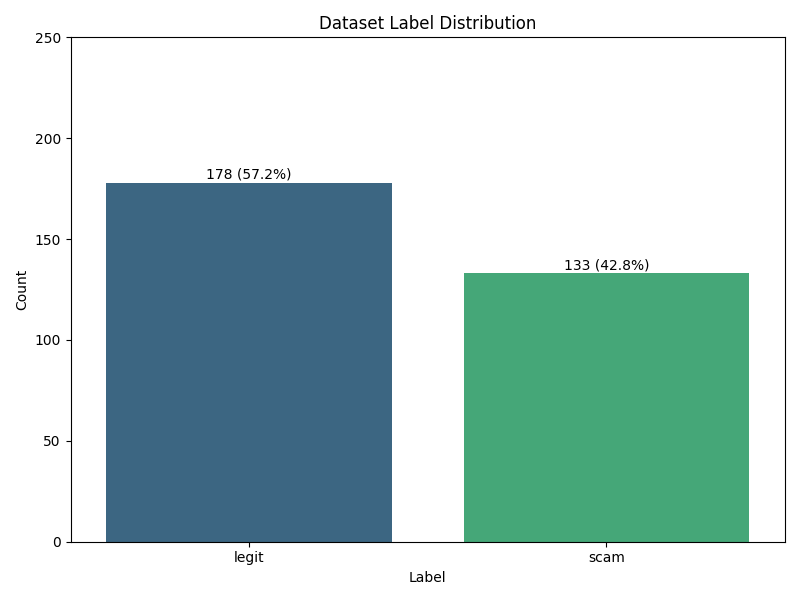
\includegraphics[width=\textwidth]{data_balancing.png}
\caption{Equilibrio delle istanze del dataset}
\end{figure}

\newpage

\begingroup%
\makeatletter%
\let\clearpage\relax% Stop LaTeX from going to a new page; and
\vspace*{\fill}%
\vspace*{\dimexpr-50\p@-\baselineskip}% Remove the initial (default) 50pt gap (plus 1 line)
\chapter{Data Modeling}
\vspace*{\fill}%
\endgroup
\newpage

\section{Introduzione al Modellamento}
In questa fase costruiremo il nostro modello, seguendo due fasi ben precise:
\begin{itemize}
    \item Scelta di tecniche e algoritmi;
    \item Addestramento del Machine Learning Model.
\end{itemize}

\section{Tecnica}
In questa fase, analizziamo il problema in esame per capire con quale tecnica creare il nostro Modello.\\
Essendo un problema in cui abbiamo bisogno di etichettare le nuove istanze che verranno date al Modello, e i dati stessi di traning sono anche essi etichettati, possiamo dedurre che questo problema è un problema di \textbf{Classificazione}, più nello specifico un problema di classificazione binaria, in quanto le etichette possono assumere solo due valori: "scam" o "legit".

\section{Algoritmi}
Per un problema di classificazione abbiamo a disposizione un gran numero su cui fare affidamento.\\
Tra di essi ne scegliamo due, in quanto vogliamo comparare quali dei due potrebbe darci migliori performance in questo ambiente:
\begin{itemize}
    \item \texttt{\textbf{Naïve Bayes}};
    \item \texttt{\textbf{Random Forest}}.
\end{itemize}
Ora, andiamo ad analizzare perchè dovremmo preferire uno dei due, all'altro.

\subsection{Naïve Bayes}
L'algoritmo Naïve Bayes è uno dei classificatori più semplici e veloci, sia in fase di addestramento che di utilizzo, grazie alla sua efficienza computazionale e al presupposto di indipendenza tra le feature. \\
Questo lo rende particolarmente adatto per problemi di classificazione con dataset piccoli o medi, dove la velocità e l'usabilità sono prioritarie. \\ 
Tuttavia, un limite significativo di Naïve Bayes è la sua assunzione di indipendenza tra le feature, che raramente è valida per dati reali. Nel contesto del problema affrontato da OverseerAI, questa limitazione è particolarmente rilevante: le feature \texttt{\color{red}{title}}, \texttt{\color{red}{description}} e \texttt{\color{red}{link\_desc}} mostrano correlazioni evidenti e devono essere analizzate in relazione l'una con l'altra per produrre risultati significativi. \\
Di conseguenza, pur essendo un algoritmo rapido ed efficiente, Naïve Bayes potrebbe non essere la scelta ottimale per problemi in cui le dipendenze tra le feature giocano un ruolo cruciale nella qualità della classificazione.

\subsection{Random Forest}
L'algoritmo Random Forest che è stato scelto per affrontare il problema di classificazione come algoritmo principale grazie alla sua capacità di gestire dataset con feature correlate.\\
Esso costruisce un insieme di alberi decisionali e combina le loro previsioni, migliorando così la robustezza e riducendo il rischio di overfitting rispetto a un singolo albero decisionale. \\
Grazie all'uso di più alberi decisionali, esso riesce anche a trovare pattern nascosti, qualità che nell'attuale problema in analisi ha grande rilevanza e utilità.\\
Queste caratteristiche hanno determinato come scelta definitiva del suddetto algoritmo per la risoluzione del problema.\\
Anche se esso richiede più risorse computazionali rispetto a algoritmi più semplici, come Naïve Bayes, il bilanciamento tra accuratezza e capacità di generalizzazione (utile ai pattern nascosti) lo rende una scelta ideale per il problema in esame.

\section{Addestramento}
Andiamo ora ad addestrare il nostro modello, usando l'algoritmo Random Forest.\\
Per praticità di utilizzo, e per fornire una demo riproducibile, il modello addestrato verrà salvato in formato .pkl, per mantenere tutto il settaggio del modello eseguito in fase di training.\\
Come primo step, scriviamo il codice che processerà il dataset e allenerà il nostro modello:
\begin{lstlisting}[language=Python]
import pandas as pd
from sklearn.model_selection import KFold
from sklearn.pipeline import Pipeline
from sklearn.compose import ColumnTransformer
from sklearn.feature_extraction.text import TfidfVectorizer
from sklearn.ensemble import RandomForestClassifier
from sklearn.metrics import accuracy_score, precision_score, recall_score
import joblib

def create_pipeline():
    preprocessor = ColumnTransformer(
        transformers=[
        ('title_tfidf', TfidfVectorizer(max_features=5000), 'title'),
        ('description_tfidf', TfidfVectorizer(max_features=5000), 'description'),
        ('link_desc_tfidf', TfidfVectorizer(max_features=5000), 'link_desc')
        ]
    )
    
    pipeline = Pipeline(steps=[
        ('preprocessor', preprocessor),
        ('classifier', RandomForestClassifier(n_estimators=100, random_state=42, class_weight="balanced"))
    ])
    
    return pipeline
\end{lstlisting}
Prima di iniziare ad addestrare il modello, abbiamo bisogno di processare i dati per renderli "capibili" al nostro classificatore, se ne occuperà il \texttt{preprocessor}.\\
In \texttt{ColumnTransformer()} trasformiamo le nostre colonne (features) in vettori numerici, utilizzando la funzione \textbf{TF-IDF} (Term Frequency-Inverse Document Frequency), che quantifica l'importanza di una parola all'interno del dataset. Il dizionario di importanza nella nostra soluzione avrà un valore arbitrario massimo di 5000 elementi.
\newpage
In \texttt{pipeline()} utilizziamo la funzione Pipeline per creare una "catena di montaggio", che eseguirà in ordine questi step:
\begin{enumerate}
    \item Esecuzione del \texttt{preprocessor};
    \item Esecuzione del classificatore \texttt{RandomForestClassifier()} con 100 alberi differenti, seed randomico (con cui si possono replicare i risultati) = 42 e un compensamento automatico per lo squilibrio delle classi nel problema di esame, dando un peso maggiore alle classi meno rappresentate.
\end{enumerate}
\hfill \break
La successiva fase utilizzerà ciò che abbiamo creato per allenare il modello, e validerà ogni istanza di allenamento eseguita.
\begin{lstlisting}[language=Python]
import # ...

def train_and_evaluate(df):
    X = df[['title', 'description', 'link_desc']]
    y = df['label']

    kf = KFold(n_splits=10, shuffle=True, random_state=42)
    fold_num = 1

    accuracy_scores = []
    precision_scores = []
    recall_scores = []
    
    for train_index, test_index in kf.split(X):
        X_train, X_test = X.iloc[train_index], X.iloc[test_index]
        y_train, y_test = y.iloc[train_index], y.iloc[test_index]

        pipeline = create_pipeline()
        pipeline.fit(X_train, y_train)
        y_pred = pipeline.predict(X_test)

        acc = accuracy_score(y_test, y_pred)
        prec = precision_score(y_test, y_pred, average='macro')
        rec = recall_score(y_test, y_pred, average='macro')
        print(f"Fold {fold_num} - Accuracy: {acc:.3f}, Precision: {prec:.3f}, Recall: {rec:.3f}")
        accuracy_scores.append(acc)
        precision_scores.append(prec)
        recall_scores.append(rec)

        fold_num += 1

    joblib.dump(pipeline, 'random_forest_model.pkl')
    print("Modello salvato come 'random_forest_model.pkl'")
\end{lstlisting}
I dati che vengono usati per l'allenamento vengono presi dal dataset e divisi in due categorie: una parte va al training, l'altra va alla validazione della fase di training.\\
Per questo processo usiamo il metodo di convalida \textbf{K-Fold N-times cross validation}.\\
Nel nostro caso \texttt{N-times = 10}, e la funzione mescola le istanze del dataset prima di dividerle in gruppi per evitare dipendenze sequenziali dei dati (e viene fornito un seed per replicare l'istanza di training).\\
Ad ogni iterazione del ciclo \texttt{for} viene eseguita la singola iterazione del \texttt{K-fold}.\\
Sapendo che \textbf{X} sono le istanze con valori title, description e link\_desc, e \textbf{y} sono le istanze con solo label come valore, all'interno del ciclo vengono assegnati valori di training e test per X e valori di training e test per y, utilizzando lo split attuale (creato usando \texttt{kf.split(X)}).\\
Si procede, dopo questa suddivisione, a creare la pipeline di preprocessamento vista in precedenza, e con \texttt{pipeline.fit()} allena il modello.\\
\texttt{y\_pred = pipeline.predict(X\_text)} cerca invece di predirre ogni valore di X\_text.\\
Successivamente, la funzione calcola le metriche di valutazione per:
\[
\text{Accuracy} = \frac{\text{TP} + \text{TN}}{\text{TP} + \text{TN} + \text{FP} + \text{FN}}
\]
\[
\text{Precision} = \frac{\text{TP}}{\text{TP} + \text{FP}}
\]
\[
\text{Recall} = \frac{\text{TP}}{\text{TP} + \text{FN}}
\]\\
Dove si usano i valori dei True Positives (TP), True Negatives (TN), False Positives (FP) e False Negatives (FN).\\
L'intenzione è massimizzare codesti valori.\\
Infine, dopo il completamento dell'esecuzione del ciclo \texttt{for}, utilizziamo la funzione \texttt{joblib.dump()} per salvare il traning e la validazione fatti come modello allenato.\\

\begin{figure}[h]
\centering
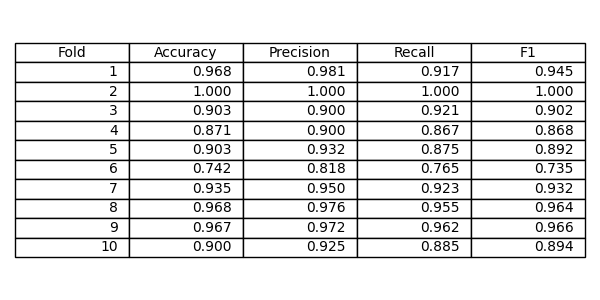
\includegraphics[width=14cm]{table.png}
\caption{Valori per-fold di Accuracy, Precision e Recall}
\end{figure}
\begin{figure}[h]
\centering
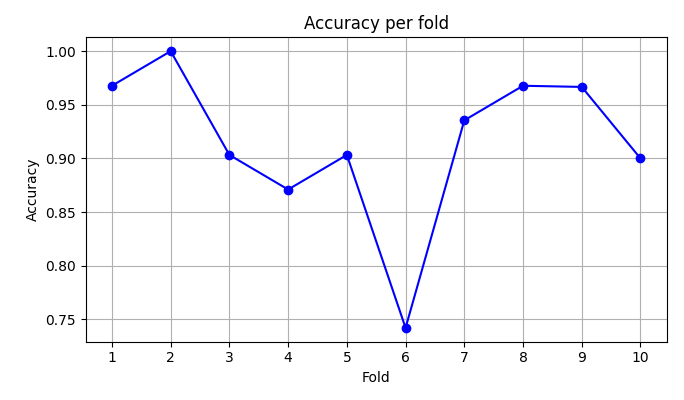
\includegraphics[width=\textwidth]{accuracy.png}
\caption{Grafico Accuracy}
\end{figure}
\begin{figure}[h]
\centering
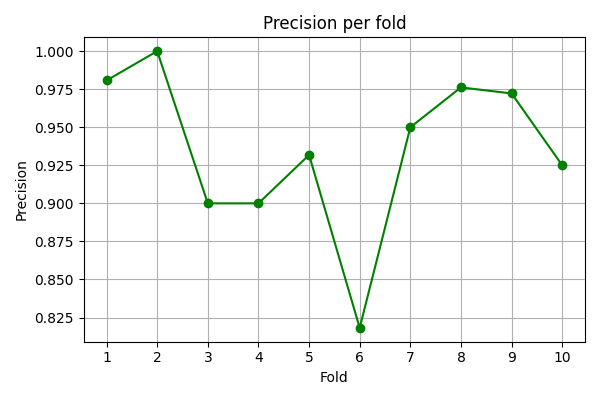
\includegraphics[width=\textwidth]{precision.png}
\caption{Grafico Precision}
\end{figure}
\begin{figure}[h]
\centering
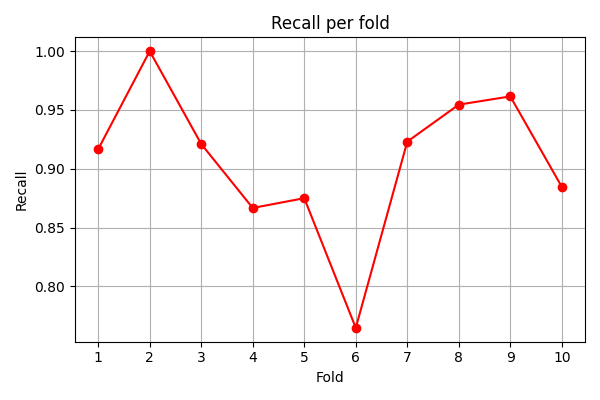
\includegraphics[width=\textwidth]{recall.png}
\caption{Grafico Recall}
\end{figure}

\end{document}
